\documentclass[crop,border=0pt]{standalone}

\usepackage{mathtools}
\usepackage{tikz}
\usetikzlibrary{positioning,scopes,arrows}

\begin{document}
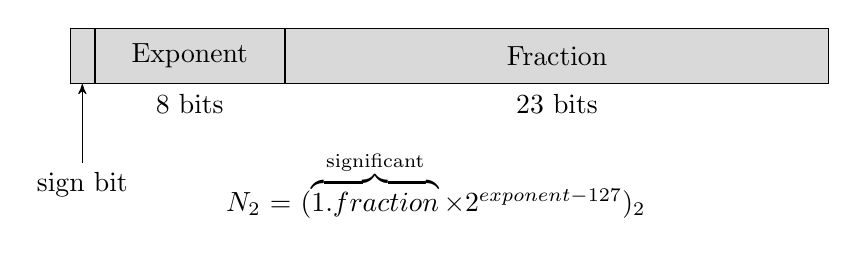
\begin{tikzpicture}[node distance=0,
  mynode/.style={draw,rectangle,fill=gray!30,align=center,inner
    sep=0,minimum height=2em},
  annotate/.style={draw=none}]

  \node [mynode, text width=3mm] (n0) {};
  \node [mynode, text width=24mm, right=of n0] (n1) {Exponent};
  \node [mynode, text width=69mm, right=of n1] (n2) {Fraction};

  \node [annotate, below=1cm of n0] (sign) {sign bit};
  \node [annotate, below=of n1] {8 bits};
  \node [annotate, below=of n2] {23 bits};

  \node [annotate, right=1cm of sign] {\(N_2\) = \((\overbrace{1.fraction}^\text{significant}\times 2^{exponent - 127})_2\)};

  {[->,>=stealth']\draw (sign) -- (n0);}
\end{tikzpicture}
\end{document}
